\section{Analysis}
\label{sec: analysis}


\subsection{feature analysis}

\begin{figure}[ht]
    \centering
    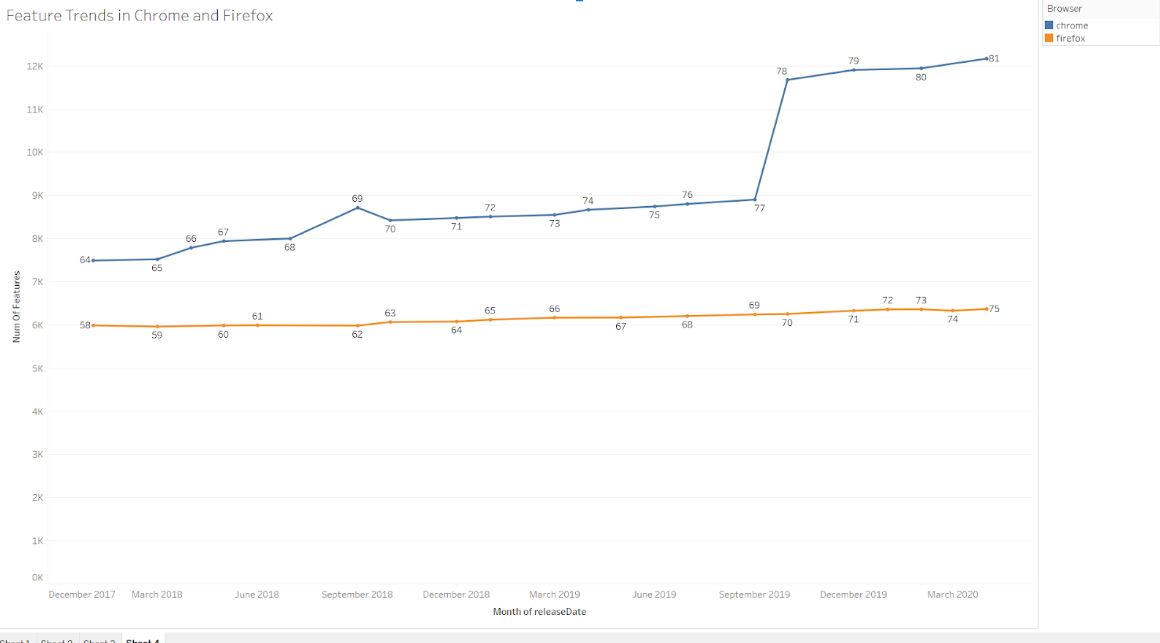
\includegraphics[width=\columnwidth]{figures/firefox-chrome-trends.png}
    \caption{Feature trends in firefox and chrome. Blue line represents number of features in chrome. Yellow line represents firefox.\ali{Need to rescale the chart so the text could be visible}}
    \label{fig:times_bar}
\end{figure}

\begin{figure}[ht]
    \centering
    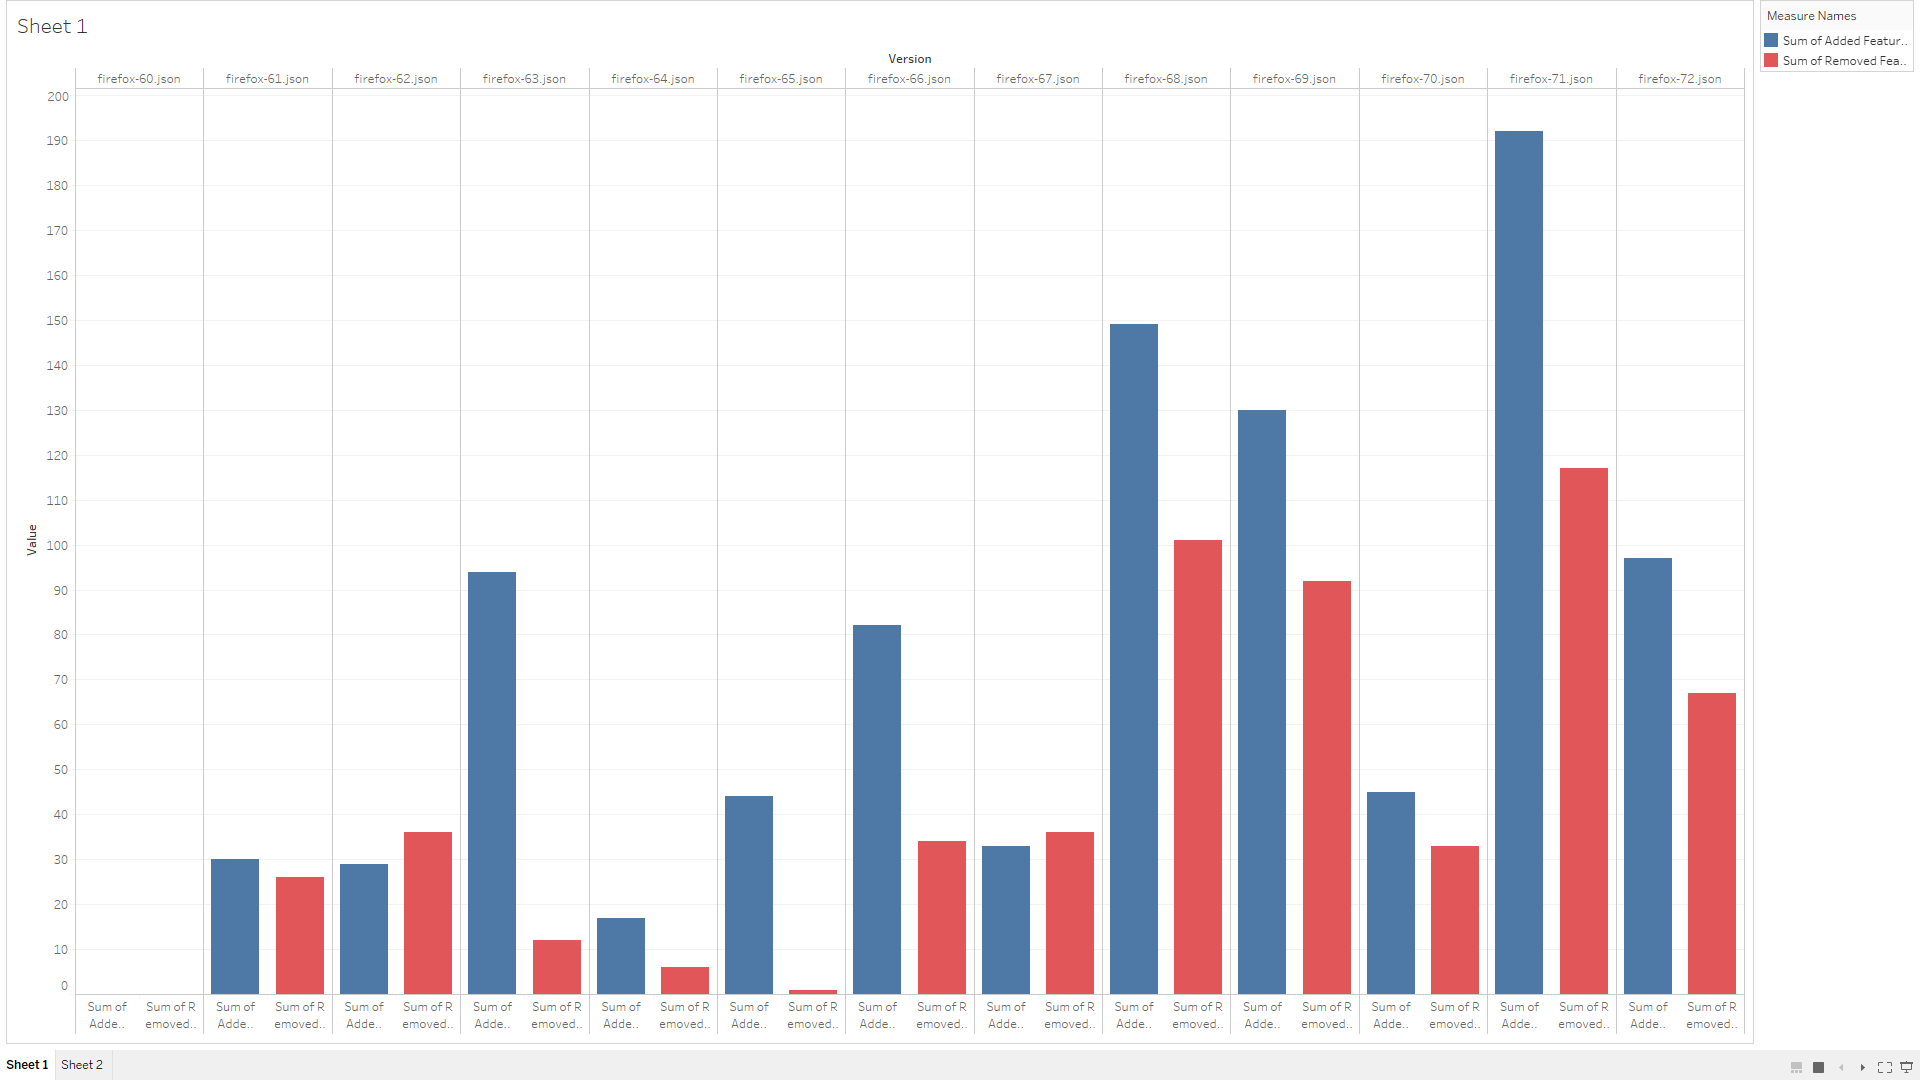
\includegraphics[width=\columnwidth]{figures/addremove-feature-trend-firefox}
    \caption{Feature Introduction and removal in Firefox. Red bars represent the removed features and the blue bars represent added features.}
    \label{fig:times_bar}
\end{figure}


\begin{figure}[ht]
    \centering
    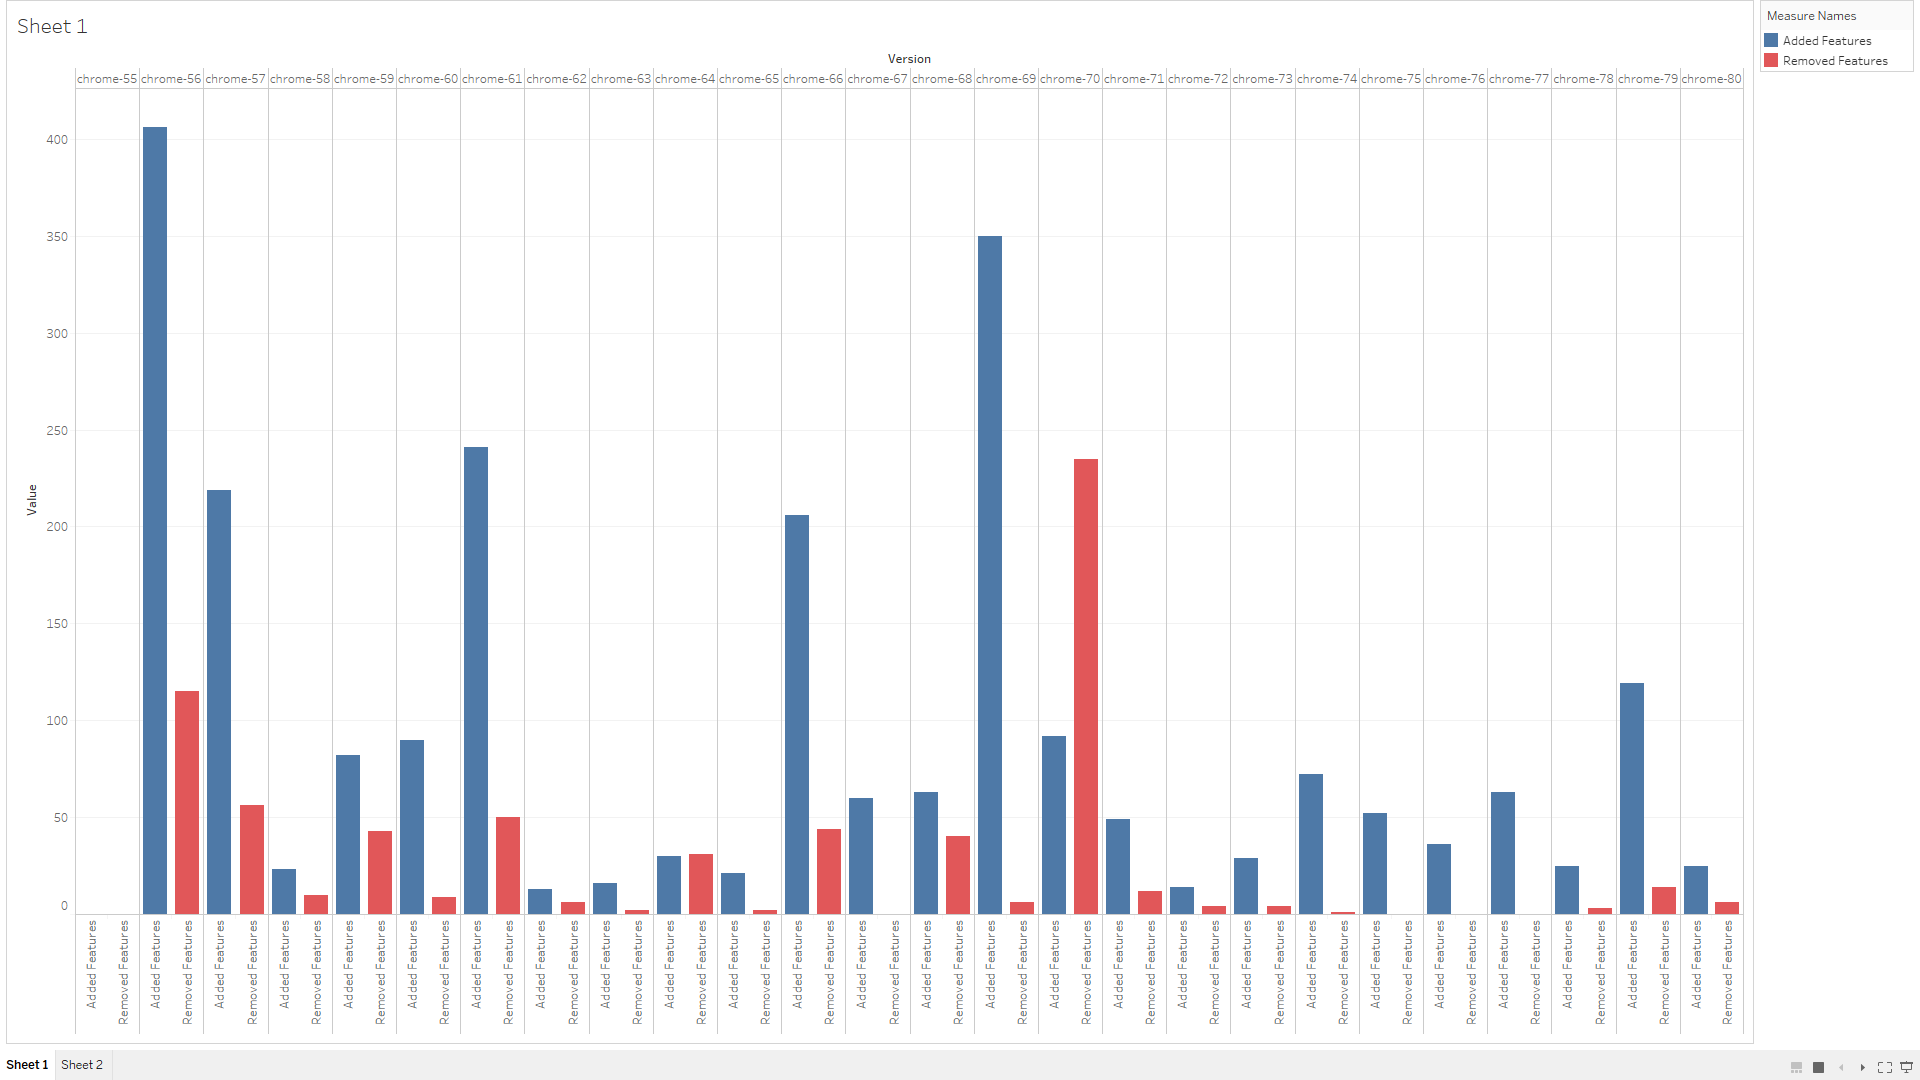
\includegraphics[width=\columnwidth]{figures/addremove-feature-trend-chrome}
    \caption{Feature Introduction and removal in Chrome. Red bars represent the removed features and the blue bars represent added features.}
    \label{fig:times_bar}
\end{figure}


\subsection{vulnerability analysis}

\ali{Still need to generate results and reports for this section.}